\chapter{Analysis}

- Scenarios


- Hard limits
    - ttl
    - stream baum vs minimal spanning tree
        - histogram

- Discussion
- scaling further
    - dht

- nucleus scenarios
    - gobble
    - eclipsed group re–joining
    - router lost
    - glare problem: two peers try to open same connection
        - circuit glare, aka dual seizure like in phone systems
        - see \cite[pp. 194-194]{signaling-systems-book}


Random Quotes:
\say{Analysis of a P2P system by Saroiu et al. [3] show that the longer a node has been up, the more likely it is to remain up for another hour.}(http://gleamly.com/article/introduction-kademlia-dht-how-it-works). IPFS bitswapping auch da hinschreiben

\section{Analysing small scenarios}
\subsection{Genesis}

\begin{figure}[htb!]
  \centering
    \subfloat[]{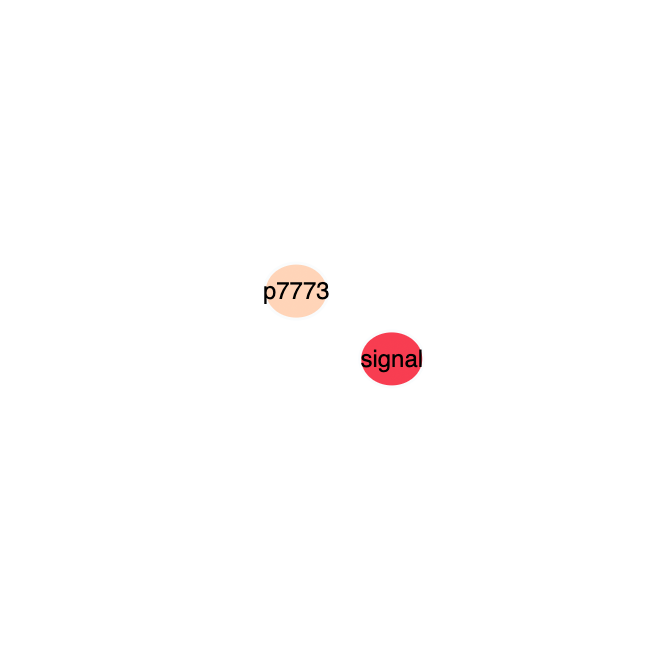
\includegraphics[width=0.33\textwidth]{graphics/analysis/mini-scenarios/become-router/1.png} 
    \label{fig:filmstrips-genesis-a}}
    \subfloat[]{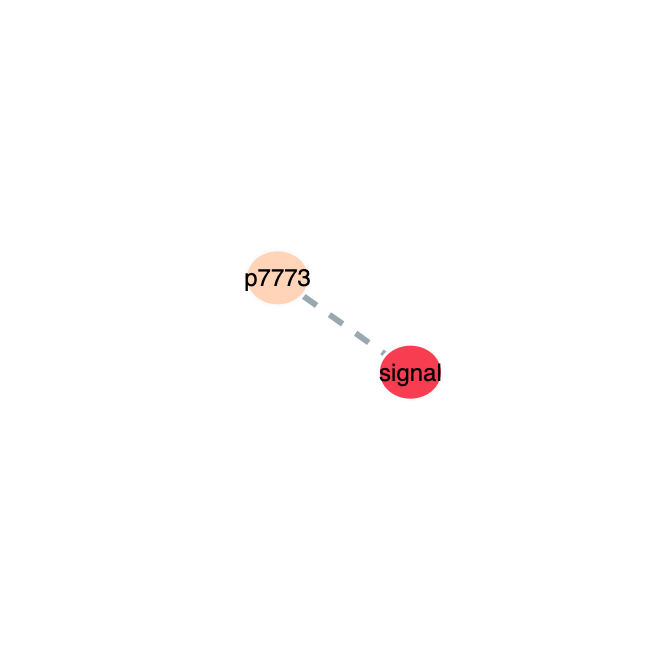
\includegraphics[width=0.33\textwidth]{graphics/analysis/mini-scenarios/become-router/2.png} \label{fig:filmstrips-genesis-b}}
	\subfloat[]{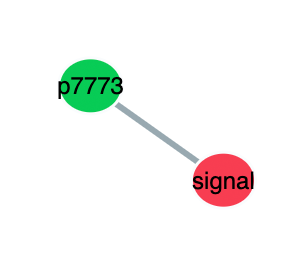
\includegraphics[width=0.33\textwidth]{graphics/analysis/mini-scenarios/become-router/3.png} \label{fig:fig:filmstrips-genesis-c}}
	\caption{Join network as first peer}
\label{fig:overlay-topologies}
\end{figure}
\subsection{Join network \rom{1}}

\begin{figure}[htb!]
  \centering
    \subfloat[]{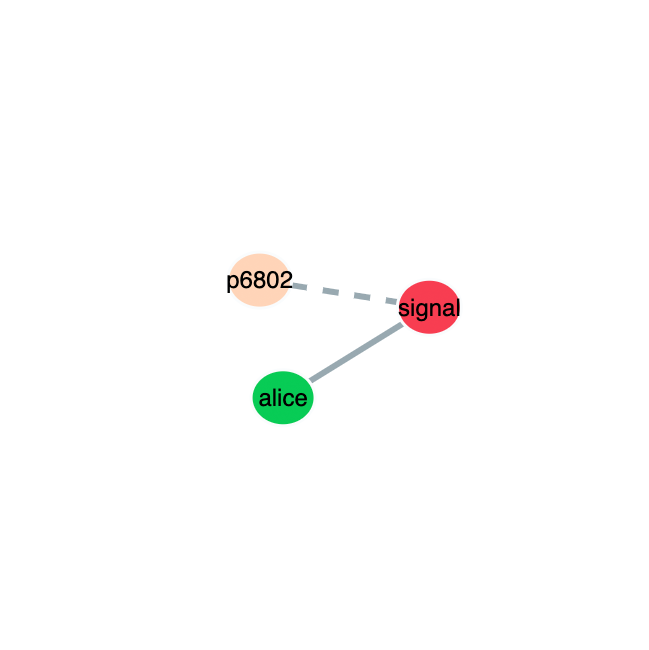
\includegraphics[width=0.25\textwidth]{graphics/analysis/mini-scenarios/join-network/1.png} \label{fig:filmstrips-join-a}}
    \subfloat[]{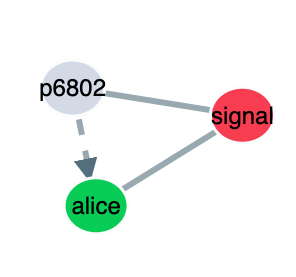
\includegraphics[width=0.25\textwidth]{graphics/analysis/mini-scenarios/join-network/2.png} \label{fig:filmstrips-join-b}}
	\subfloat[]{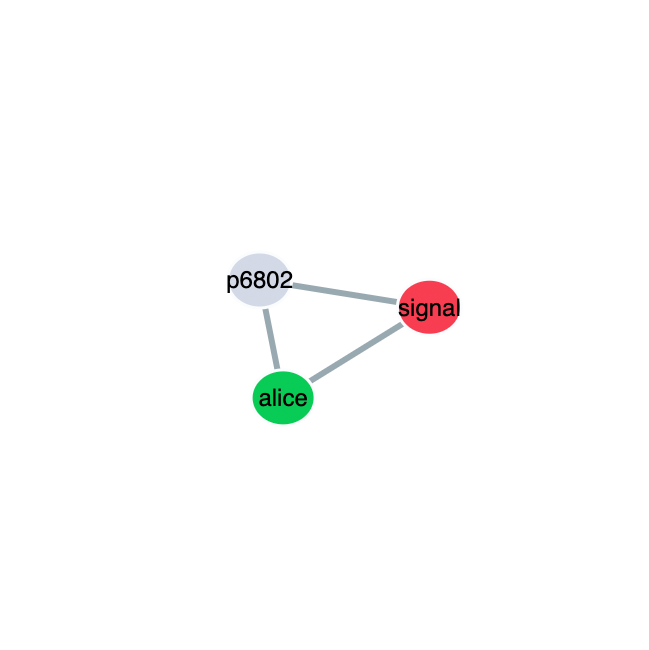
\includegraphics[width=0.25\textwidth]{graphics/analysis/mini-scenarios/join-network/3.png} \label{fig:filmstrips-join-c}}
	\subfloat[]{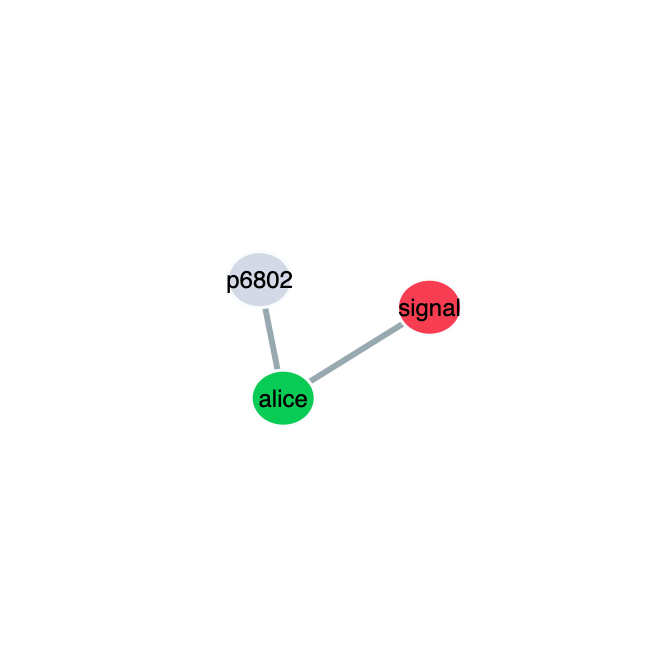
\includegraphics[width=0.25\textwidth]{graphics/analysis/mini-scenarios/join-network/4.png} \label{fig:filmstrips-join-d}}
	\caption{Join network as second peer}
\label{fig:filmstrips-join}
\end{figure}

In this scenario a second peer is joining the network. As described in the in the \textit{Genesis} scenario it opens a connection to the \signal peer (\vref{fig:filmstrips-join-a}). This time the \signal peer already knows a \router peer—\alice. Therefore, it only upgrades the \newbie peer to the role \peer. Also it sends a \peerUpdate to the new peer in order to let it update its peer table. 

A peer with the role \peer has always the desire to satisfy its connection goal.
Thus, its next intention is to open connections to as many peers as it knows, until its connection goal is satisfied. As it only knows the reported peer \alice it is trying to connect to her by sending a connection offer via the \signal peer (\vref{fig:filmstrips-join-b}).

\alice has connections available, hence she is accepting the connection offer with an answer, that is again delivered via the \signal. As soon as the new peer receives the answer, it establishes the connection to \alice (\vref{fig:filmstrips-join-c}).

In the last step it closes the connection to the \signal peer because it knows a peer with the role \router (\vref{fig:filmstrips-join-d}).


\subsection{Join network but router is already full of capacity}

\begin{figure}[htb!]
  \centering
    \subfloat[]{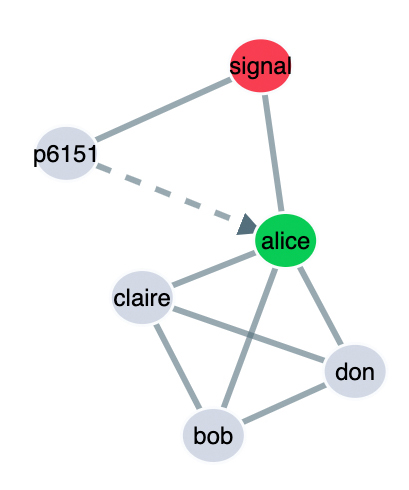
\includegraphics[width=0.33\textwidth]{graphics/analysis/mini-scenarios/router-full-redirect/1.jpg} \label{fig:filmstrips-redirect-a}}
    \subfloat[]{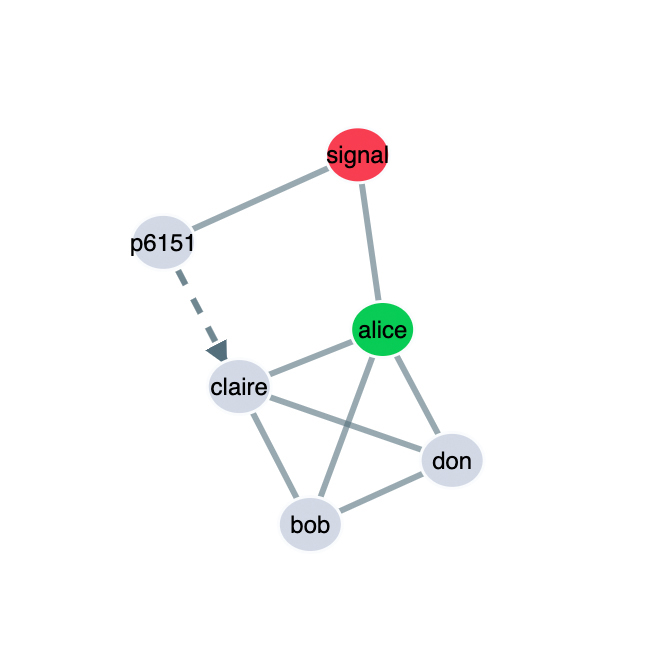
\includegraphics[width=0.33\textwidth]{graphics/analysis/mini-scenarios/router-full-redirect/2.jpg} \label{fig:filmstrips-redirect-b}}
	\subfloat[]{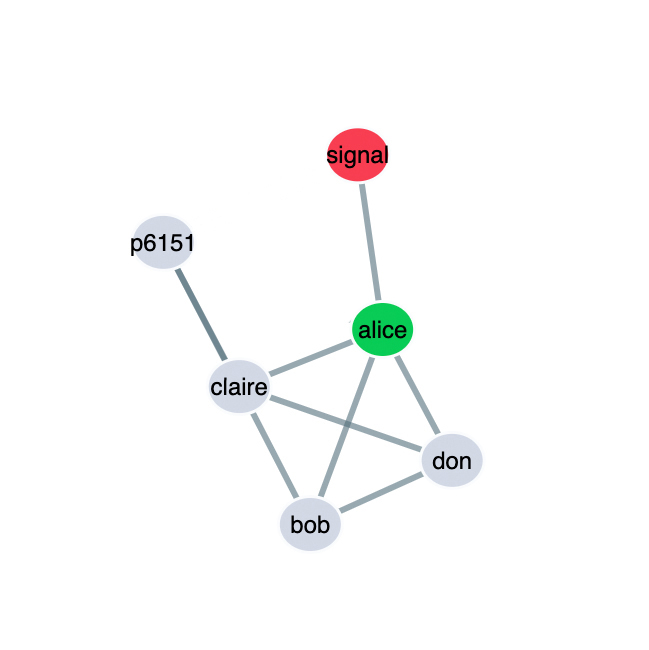
\includegraphics[width=0.33\textwidth]{graphics/analysis/mini-scenarios/router-full-redirect/3.jpg} \label{fig:filmstrips-redirect-c}}
	\caption{Join network peer}
\label{fig:overlay-topologies}
\end{figure}
\subsection{Bottleneck prevention}

\begin{figure}[htb!]
  \centering
    \subfloat[]{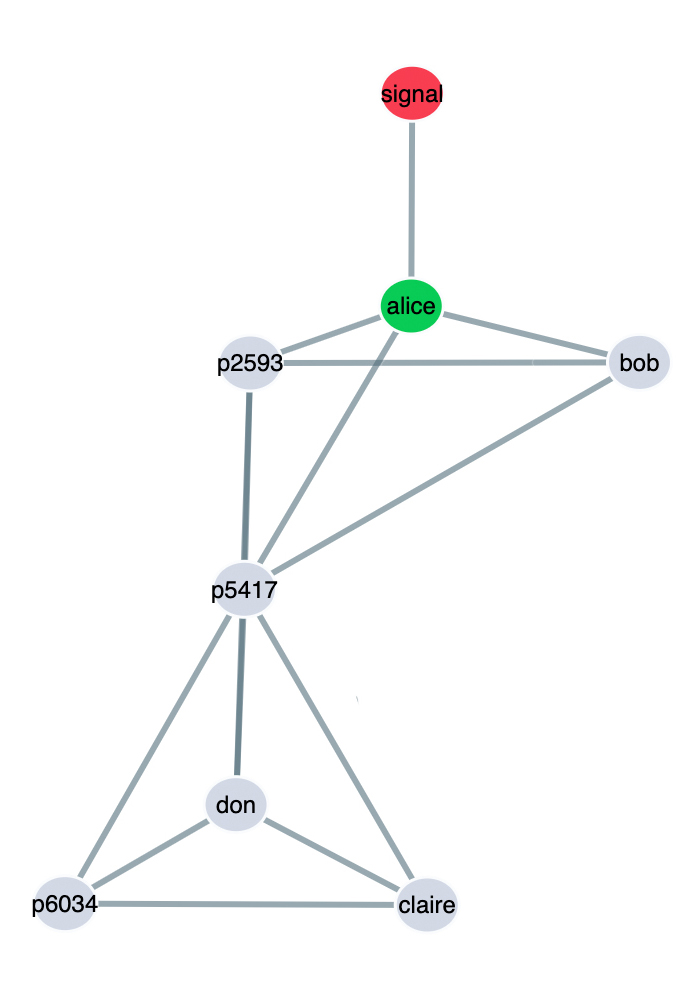
\includegraphics[width=0.33\textwidth]{graphics/analysis/mini-scenarios/bottleneck-prevention/1.jpg} \label{fig:filmstrips-bottleneck-prevention-a}}
    \subfloat[]{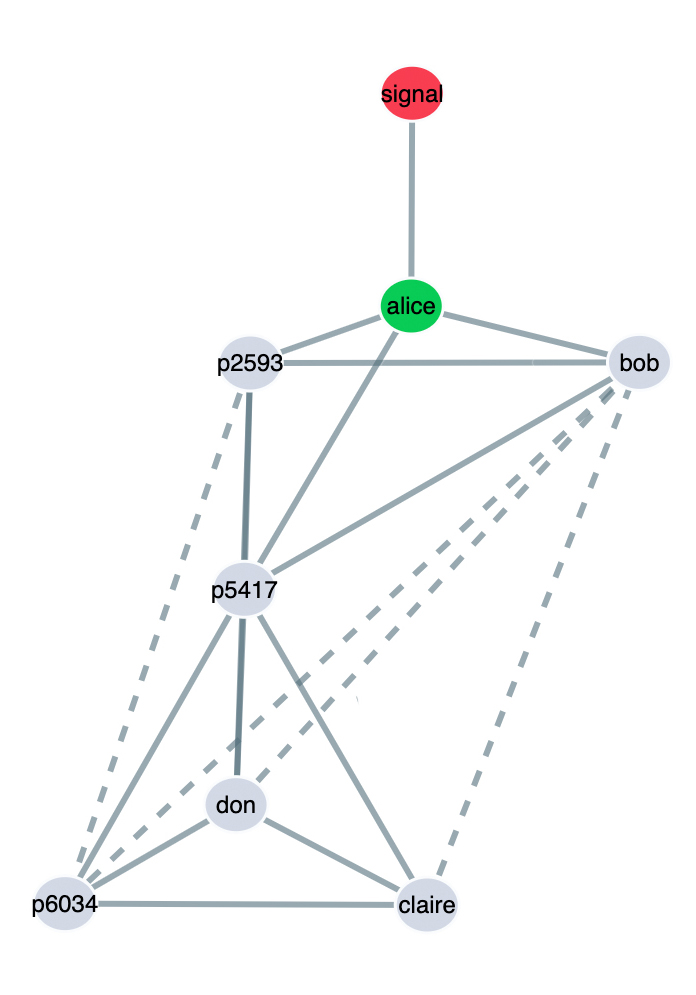
\includegraphics[width=0.33\textwidth]{graphics/analysis/mini-scenarios/bottleneck-prevention/2.jpg} \label{fig:filmstrips-bottleneck-prevention-b}}
	\subfloat[]{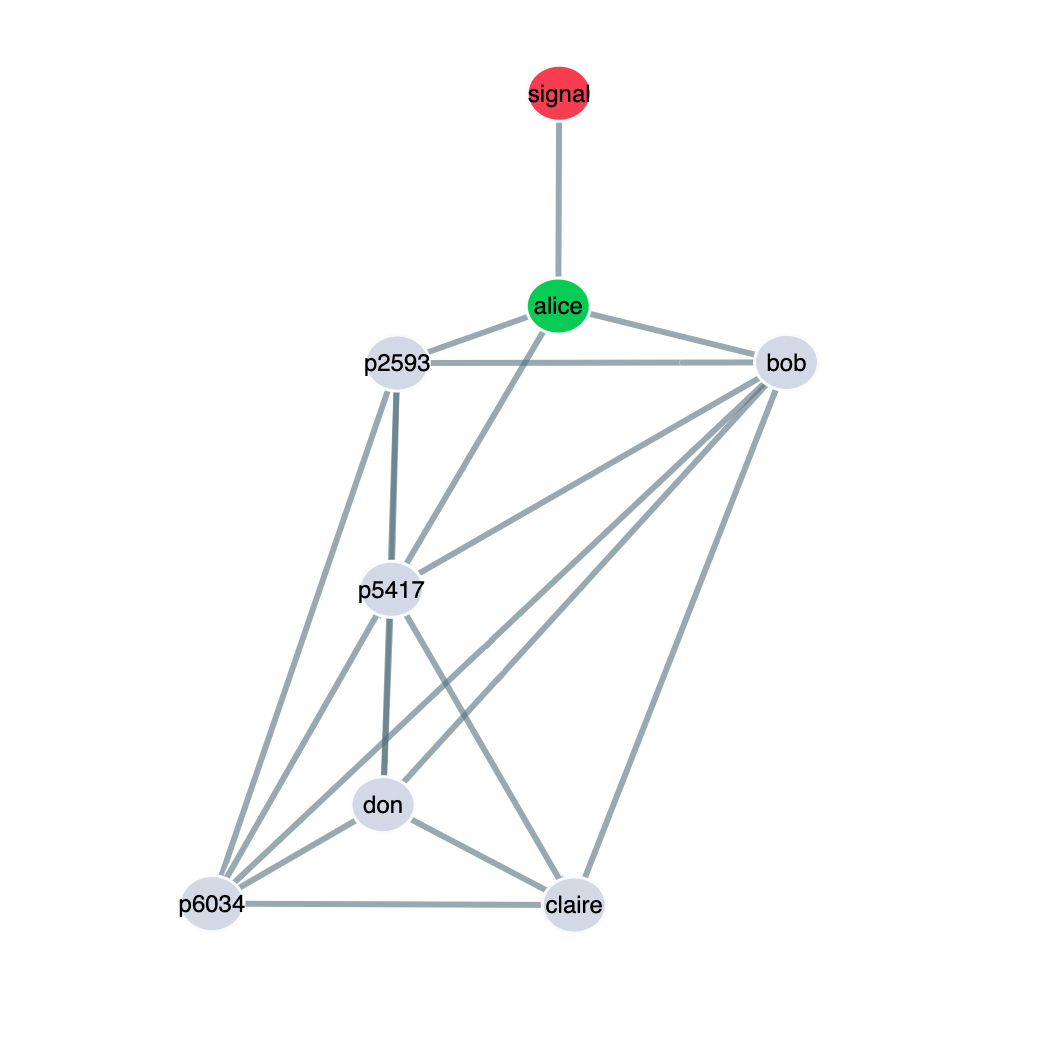
\includegraphics[width=0.33\textwidth]{graphics/analysis/mini-scenarios/bottleneck-prevention/3.jpg} \label{fig:filmstrips-bottleneck-prevention-c}}
	\caption{Preventing a bottleneck}
\label{fig:overlay-topologies}
\end{figure}
\subsection{Send message}

\begin{figure}[htb!]
  \centering
    \subfloat[]{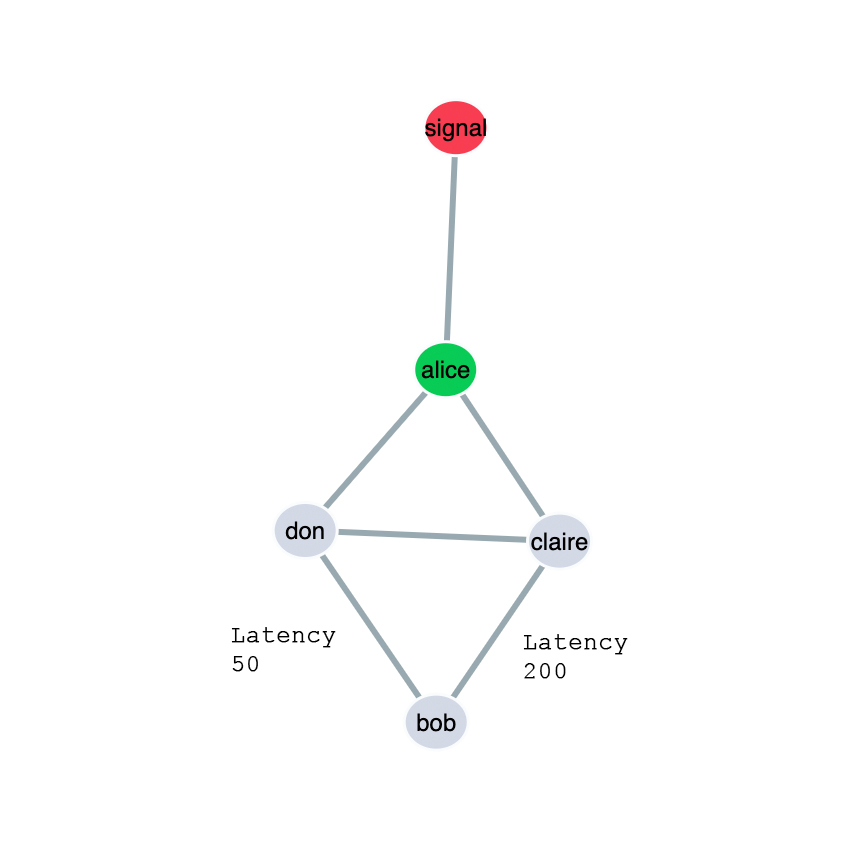
\includegraphics[width=0.25\textwidth]{graphics/analysis/mini-scenarios/send-message/1.jpg} \label{fig:filmstrips-send-message-a}}
    \subfloat[]{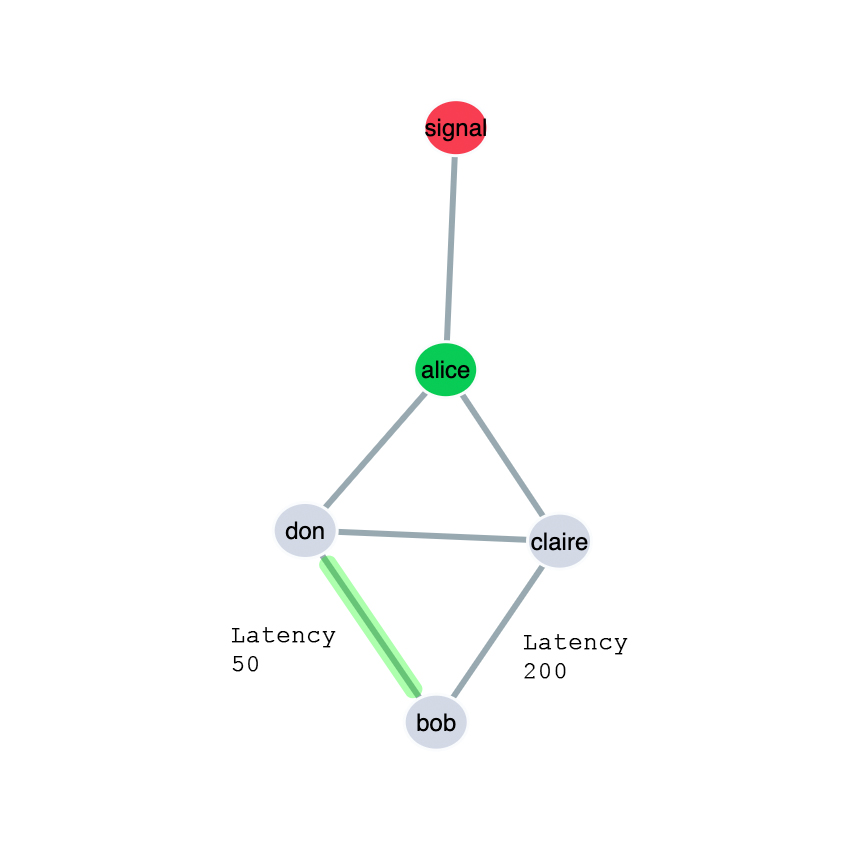
\includegraphics[width=0.25\textwidth]{graphics/analysis/mini-scenarios/send-message/2.jpg} \label{fig:filmstrips-send-message-b}}
	\subfloat[]{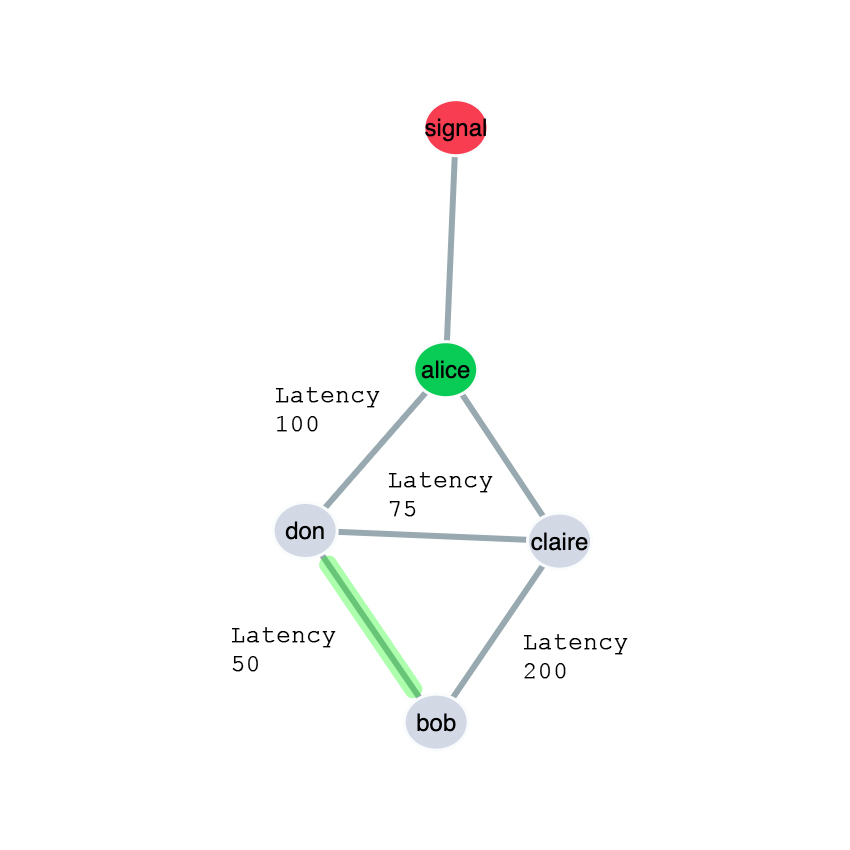
\includegraphics[width=0.25\textwidth]{graphics/analysis/mini-scenarios/send-message/3.jpg} \label{fig:filmstrips-send-message-c}}
	\subfloat[]{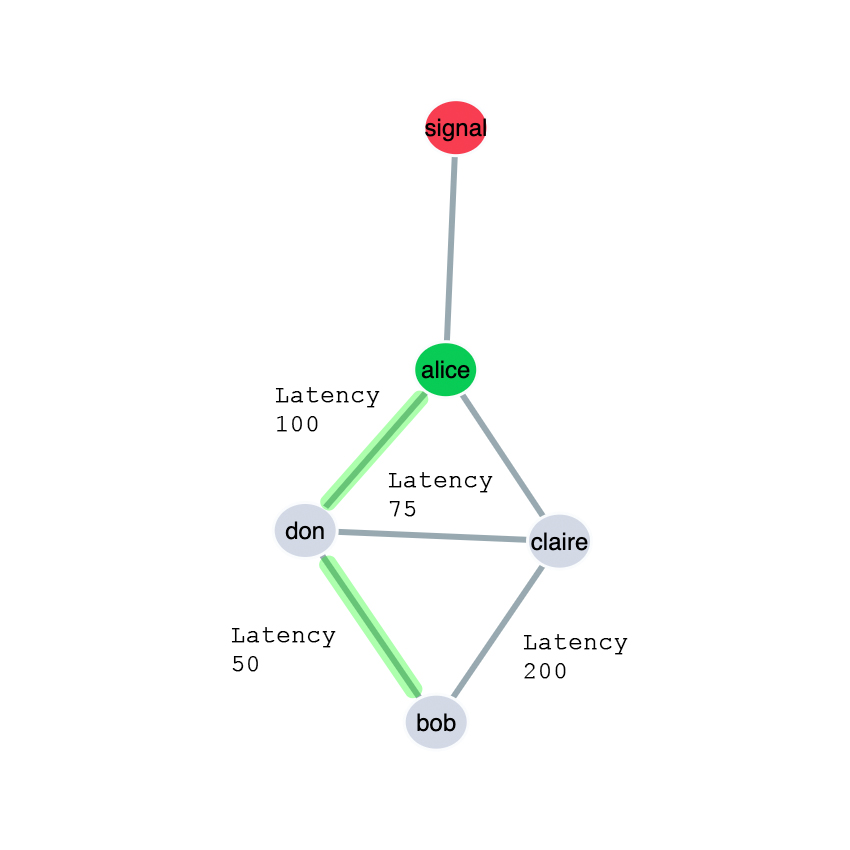
\includegraphics[width=0.25\textwidth]{graphics/analysis/mini-scenarios/send-message/4.jpg} \label{fig:filmstrips-send-message-d}}
	\caption{Path of a message}
\label{fig:overlay-topologies}
\end{figure}
\subsection{Broadcast}

\begin{figure}[htb!]
  \centering
    \subfloat[]{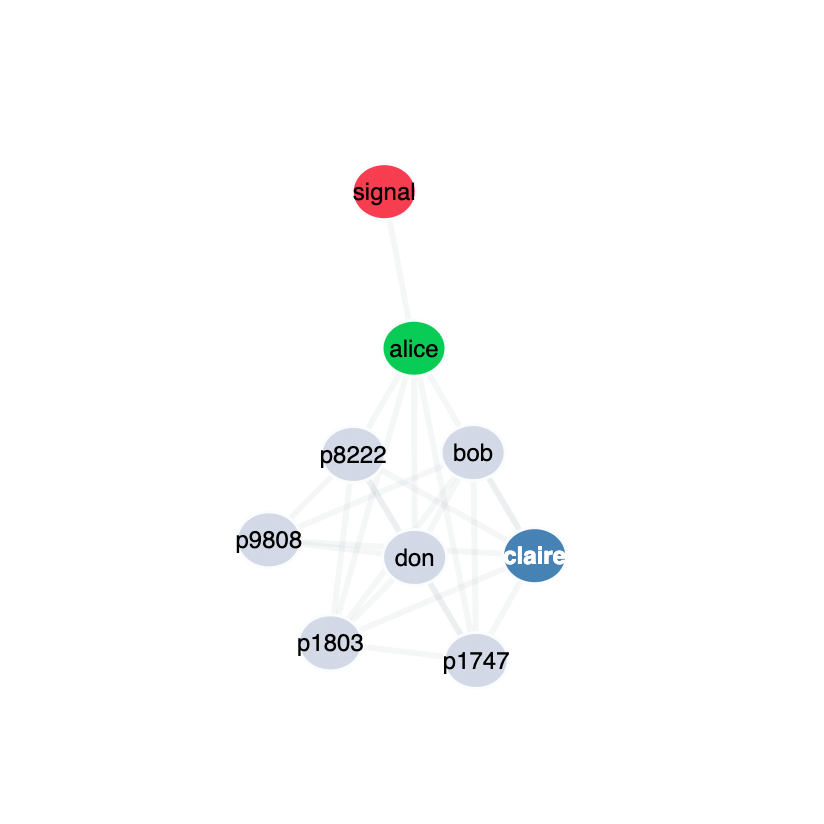
\includegraphics[width=0.25\textwidth]{graphics/analysis/mini-scenarios/stream/1.png} \label{fig:filmstrips-broadcast-a}}
    \subfloat[]{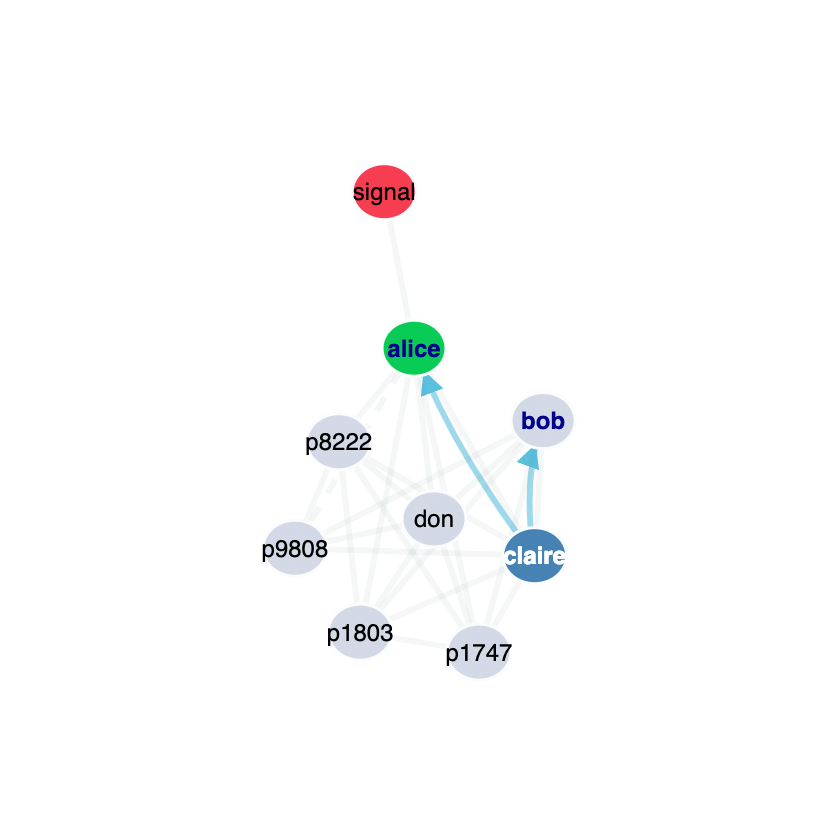
\includegraphics[width=0.25\textwidth]{graphics/analysis/mini-scenarios/stream/2.png} \label{fig:filmstrips-broadcast-b}}
	\subfloat[]{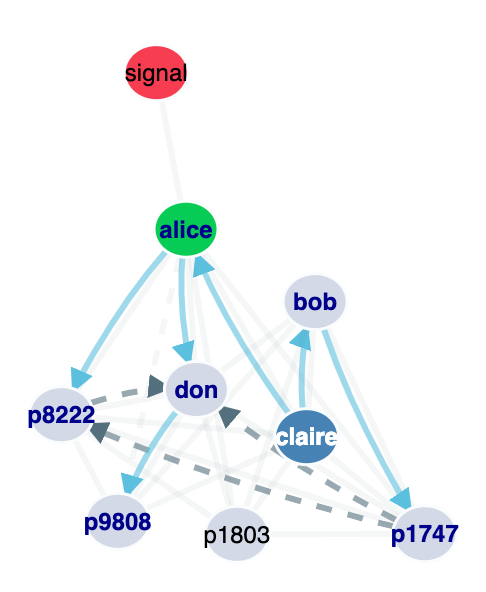
\includegraphics[width=0.25\textwidth]{graphics/analysis/mini-scenarios/stream/3.png} \label{fig:filmstrips-broadcast-c}}
	\subfloat[]{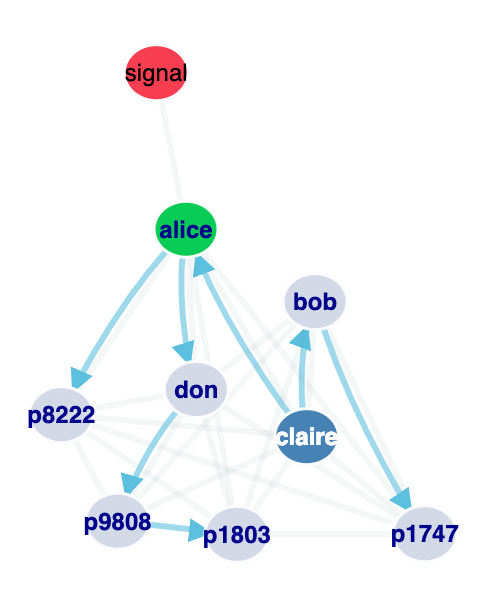
\includegraphics[width=0.25\textwidth]{graphics/analysis/mini-scenarios/stream/4.png} \label{fig:filmstrips-broadcast-d}}
	\caption{Broadcasting tree creation}
\label{fig:overlay-topologies}
\end{figure}
\newpage
\input{content/6-analysis/2-meshing.tex}
\newpage
\section{Streaming Analysis}

\subsection{Topology}

Since video streams over \gls{webrtc} connections decrease in quality per hop, as discussed in \vref{TOOD}, an optimal streaming topology would would be a \textit{perfect k–ary tree}, given nodes can upload $k$ streams simultaneously. A perfectly balanced binary tree, for example, would be the optimal streaming topology for $k=2$.

As the streaming topology is built on the collective knowledge of the overlay network, it depends heavily on the state the overlay mesh has reached at the point the stream is started. It must also be considered, that the streaming tree is constructed in the two phases detailed in \vref{TODO}. The push phase aims at achieving availability fast and does not regard tree balance.
It is also important to note, that due to node churn, the stream topology can change unexpectedly as nodes try to re–acquire a connection to a source provider.

The quality of the streaming topology is inspected in a churn–free simulation setup. Given a scenario of $n=100$ nodes and $t=1500$ ticks a stream is automatically started at $t_{500}$. The network constructs its stream topology and the active stream connections are queried at the end of the scenario. The topology is traversed and the distance to the stream source is extracted from every node. For simplicity, the connections are handled unweighted and just the hop count is considered.
Using different random seeds, multiple runs are averaged using the mean node count per distance.

\vref{fig:streaming-topology-histogram} shows the results of the hop distribution for streaming topologies for $k=2$ and $k=3$. For comparison, the histogram also shows the distribution in an optimal binary and ternary tree given $n=100$ nodes.

\begin{figure}
\centering
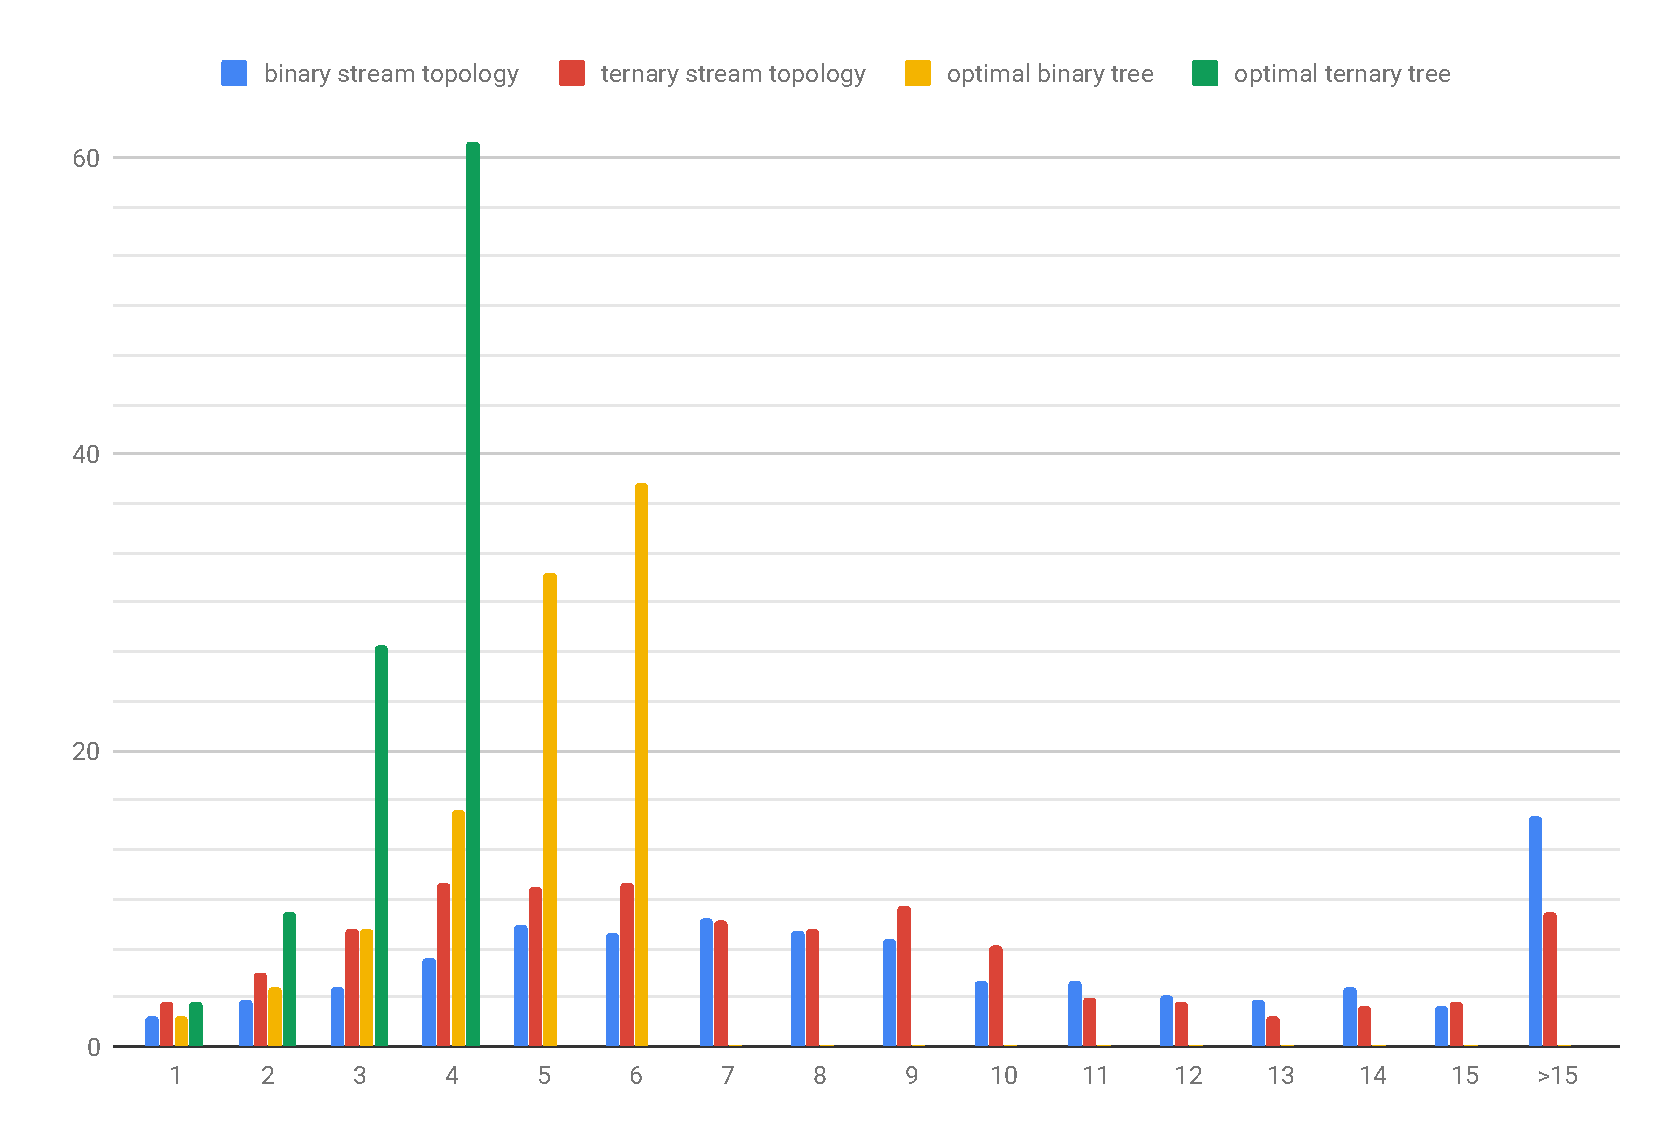
\includegraphics[width=1\textwidth]{graphics/analysis/streaming-topology-histogram.pdf}
\caption{Stream consumers per distance from stream source}
\label{fig:streaming-topology-histogram}
\end{figure}

It is evident, that the trees constructed by the overlay mesh are far from the perfectly balanced trees. A binary tree with $n=100$ nodes would not exhibit hop distances beyond $6$ and a ternary tree would not exceed distances of $4$. The respective streaming trees show a much broader distribution. The spikes caused behind the quadratic/cubic function of the optimal trees, are not to be found in the stream topologies. Yet, half the nodes exceed $8$ connection hops for $k=2$ and half the nodes for $k=3$ are above $6$ connections away from the source.

This non–optimal distribution can be explained by collisions during the push phase. As multiple nodes in the same radius around the stream source receive the channel, they try to push it out to their most reliable neighbour. However, chances are, their own best neighbour is also the choice of some other node on the same radius. As a result, this popular choice receives two connection offers, accepts only one and leaves the other offerer as a leaf node in the tree. While this is not a desirable state, the topology can self–heal during the pull phase. As nodes join or become interested in the channel, they will seek providers and can attach to the aforementioned leaf node.

So, in a second experiment, a more realistic scenario is set up. Nodes are not instantiated at once, but keep joining at a rate of $1/t$ to a total number of $n=50$. After half the nodes have joined the mesh, the stream is automatically started. \vref{fig:streaming-later-join} shows how the hop distances are distributed when nodes are continuously joining instead of being initiated before the stream start.

\begin{figure}
\centering
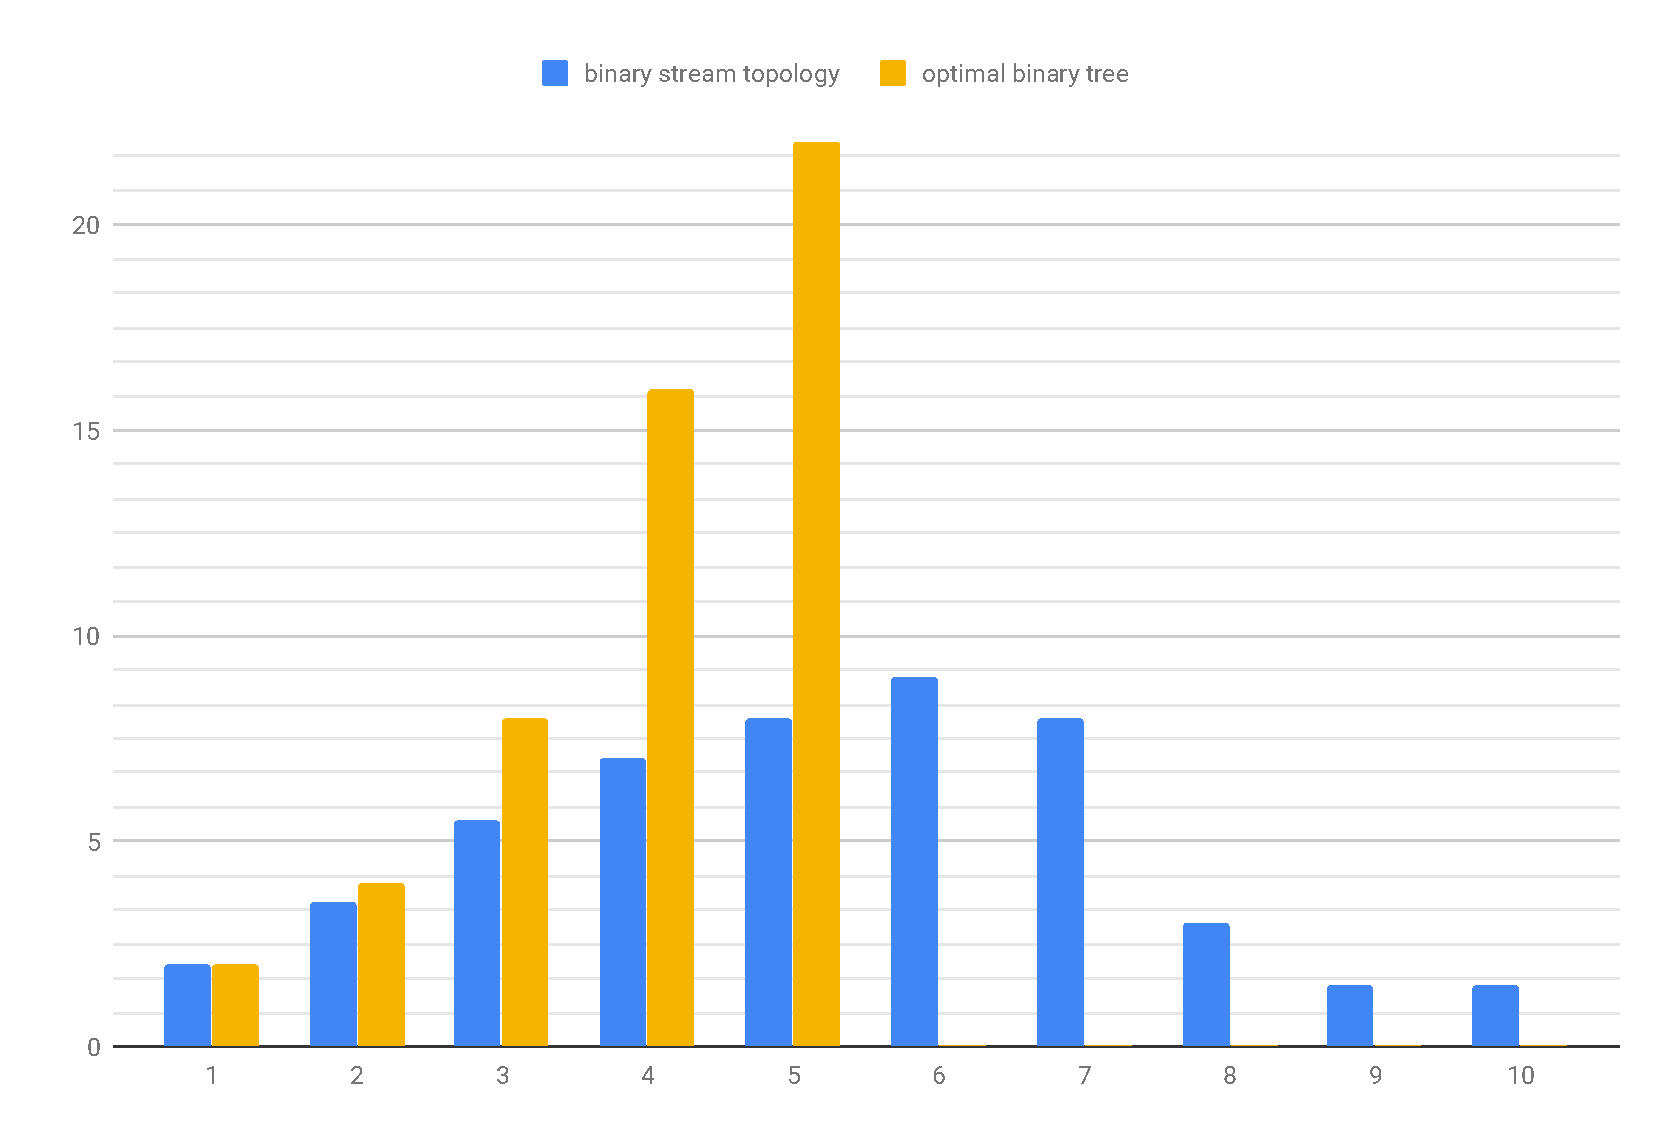
\includegraphics[width=1\textwidth]{graphics/analysis/streaming-topology-continuous-histo.pdf}
\caption{Stream consumer distance in continuous join rate scenario}
\label{fig:streaming-topology-continuous-histo}
\end{figure}

In summary, the streaming topology is heavily dependent on the underlying mesh size and structure. To cope with larger numbers of stream consumers, the system would have to perform tree optimisation. Whether this is feasible, however, depends on the application dynamics. If video channels are long–lasting and audiences are large, it would be worthwhile. If video channels are only alive a few minutes and audiences are usually small, tree optimisation would not be worth the extra negotiation effort.

\newpage
\section{Security Considerations}

\subsection{Encryption}
Whether end–to–end encrypted video streams are required, depends on the use case of the application. In a personal video chat application or the delivery of copyrighted material, it will be imperative to prevent unauthorised access to the material. However, in a publicly broadcasting application, where anyone is allowed to consume the media, end–to–end encryption will be less important.

In a \gls{p2p} delivery network, closed–audience use cases will contradict the core benefits. Why should other nodes contribute bandwidth to channels that are only viewable by closed audiences and not themselves? A more suitable application would be a \gls{p2p} multi–cast scenario, in which aiding nodes directly benefit if traffic is routed through them. It is possible to secure multi–casting with group–bound keys that are re–negotiated on node churn \cite{ip-multicast-sec}. However, that limits the size of the \gls{p2p} network to the size of the group, given that peers should directly benefit from the bandwidth they provide.

It can still be desirable to secure traffic between nodes, for instance, to disguise which channel is being consumed by which node. Yet, this would also require to obfuscate routing paths \cite[\S4]{tor-privacy} or add deceptive traffic \cite{swarm-screen}. Again, these measures are up to the application use case to justify.

On the transport layer, the \gls{webrtc} browser stack already provides mandatory media encryption using \gls{srtp} and a secure key exchange via \gls{dtls} \cref{par:webrtc-stack}. With this encryption, the transmission channel between two nodes is secured. However, since the Mitosis implementation actively pushes the streams to any interested node, the video channel is exposed by design and the encryption ineffective. If a channel where to be restricted to a closed audience, the video stream would need to be encrypted in the application layer and transported via \gls{sctp} instead. Although modern browsers provide a low–level cryptography \gls{api} this would certainly put extra strain on end–user devices. Additionally, a group key exchange would have to be secured – all in accordance with the golden rule of cryptography: \textit{Don't roll your own crypto} \cite{motherboard-dont-roll-your-own-crypto, schneider-dont-roll-your-own-crypto}.
With that in mind, it remains up to the application semantics to justify end–to–end encryption per use–case.

\subsection{Integrity}
Apart from restricting access with encryption, a video streaming application may need to protect against identity and content forgery. The current implementation of Mitosis guarantees neither. Looking at identity generation in S/Kademlia \vref{par:kademlia} and \gls{ipfs} \vref{chap:IPFS}, it has been explored to let nodes create their own identity with asymmetric keys and a self–certifying ids. Inflationary node generation is hindered by crypto puzzles and incentives for persistent identities. From an application perspective, it is complex problem to tie node identity to the identity of the human user in a distributed system. The blockchain and \gls{iam} community are pushing to implement decentralised identity systems using smart contracts \cite{eth-identity} and identity wallets \cite{gartner-iam}.
Once a system has established a trustworthy identity management, it can also provide content integrity guarantees. By letting a content producer digitally sign its work, others can verify that the content has not been tampered with. As \citet[\S7]{anatomy-personalized-livestreaming} demonstrate, an unsecured video transmission is easily intercepted and modified. Although this sort of attack is not directly harmful to viewers, it can still impact system performance and user experience.

\subsection{Vulnerability}
Distributed \gls{p2p} networks have the advantage of lacking a \textit{central point of failure}. This makes them more resilient against denial of service attacks by design. However, there are still common vulnerabilities in these systems, that have been observed in the wild and explored in related research.
\begin{itemize}
    \itembf{Eclipse Attack} \gls{p2p} networks where nodes can influence their own position (connections) can suffer from eclipse attacks \cite[\S3]{s_kademlia}. An adversary would create nodes and place them between the victims and the rest of the network. The victims can then be cut off from communications and would need to detect the attack themselves. In this implementation, nodes are continuously evaluating their neighbours and would report back to the signal if cut off from the network. Similarly, eclipsing nodes on the video streaming layer would push them towards seeking new connections. The eclipse attack would consequently work in the Mitosis network, yet only temporarily.
    \itembf{Sybil Attack} This attack tries to manipulate a reputation system in a \gls{p2p} network by creating enough artificial nodes. \citet[via BM08]{sybil-attack} shows it can be prevented by centralised certificate authorities or placing a computational price on creating new nodes, i.e. expecting proof of work. The Mitosis network is vulnerable to this attack, as node creation is unrestricted and the reporting of peer qualities is only validated by the connection quality of the reporting node. Nodes could easily be tricked into abandoning a connection if enough of its neighbours were malicious.
    \itembf{DDoS} Distributed denial of service attacks apply to \gls{p2p} as well as any other computer network \cite[\S2]{p2p-vulnerabilities}. As Mitosis relies on \gls{webrtc} connection negotiation to traverse \gls{nat} and firewall restrictions, \textit{out of protocol} attacks on nodes are unlikely. Within the protocol, nodes are certainly exposed to attackers flooding them with messages. The system however restricts the range of messages with \gls{ttl} settings. Further, steps to protect against this class of attacks would be to limit the rate at which messages are accepted or require the solution to a \textit{crypto puzzle} for each message.
\end{itemize}
